% pdflatex rapport.tex; pdflatex rapport.tex; pdflatex rapport.tex
\documentclass[a4paper]{article}

\usepackage[francais]{babel}
\usepackage[utf8]{inputenc}
\usepackage{amsmath}
\usepackage{amssymb}
\usepackage{graphicx}
\usepackage{url}
\usepackage{subfigure}

% shorten margin
\usepackage[]{fullpage}

\title{Création d'un framework pour des routeurs
	avec support pour notification de vitesse explicite
	(kernel space)\\Tuteur : Dino LOPEZ}
\author{Mathieu BIVERT, François CHAPUIS, 
\\Calypso PETIT, Sophie VALENTIN}

\makeatletter
\def\thickhrulefill{\leavevmode \leaders \hrule height 1pt\hfill \kern \z@}
\def\maketitle{%
  \null
  \thispagestyle{empty}%
  \vskip 1cm
  \begin{center}
        \normalfont\large\huge\@author
  \end{center}
  \vfil
  \vfil
  \vfil
  \vfil
  \vfil
  \vfil
  \vfil
  \vfil
  \vfil
  \hrule height 2pt
  \par
  \begin{center}
        \huge \strut \@title \par
        \@date
  \end{center}
  \hrule height 2pt
  \par
  \vfil
  \vfil
  \vfil
  \vfil
  \vfil
  \vfil
  \vfil  
  \vfil  
  \vfil
  \vfil  
  \vfil
  \vfil
  \vfil
  \vfil  
  \vfil  
  \vfil
  \vfil  
  \vfil  
  \vfil
  \vfil
  \vfil
  \vfil
  \vfil
  \vfil
  \vfil
  \null
\begin{figure}[!ht]
        \centering
        
\includegraphics[scale=.5]{polytech.png}
\end{figure}
\vfil
\cleardoublepage
}
\makeatother

\begin{document}
\maketitle

\newpage
\tableofcontents

\newpage
\section{Introduction}

Tous les réseaux de type Ethernet nécessitent un contrôle de congestion. En effet,
l'augmentation du trafic, et la distribution non-équitable des ressources 
entre les usagers, peuvent conduire dans le meilleur des cas à un
ralentissement des communications et dans le pire des cas à des \textit{congestion collapses}.
La clé du succès de l'Internet est la mise en place du contrôle de congestion.

Une famille de protocoles de contrôle de congestion est l'ERN
(Explicit Rate Notification) \cite{thesis1}. Ils reposent sur les informations
envoyées/calculées par des routeurs, comme le taux d'émission
optimal. 

Dans le cadre de notre projet, nous devons élaborer un
module noyau à destination d'un routeur supportant l'ERN.
Un tel module établira des statistiques sur les paquets ERN\footnote{Un paquet ERN est en fait 
un paquet TCP avec des champs additionnels (dans les options TCP). Ces champs additionnels sont : 
le DrdRate (Desired Rate), le RTT (Round-trip delay time) et le cwnd (valeur courante de la fenêtre de congestion)}
qui traversent le routeur. 

Dans un premier temps, nous allons préciser
la problématique du sujet et l'outil principal utilisé. Puis, dans un
second temps, nous présenterons les solutions mises en \o euvre pour 
l'élaboration des statistiques et leurs résultats. Enfin, nous conclurons sur ce qui a été fait
et ce qu'il reste à faire.

\section{Description du problème}
\subsection{Contexte}
Un routeur est une machine qui assure l’acheminement des données,
d'un réseau informatique à un autre. Son rôle consiste à diriger
les paquets d'une interface réseau vers une autre par le meilleur chemin\footnote{Le meilleur chemin est défini par
les politiques de routage. Il peut s'agir du chemin le plus court, le plus fiable ou le plus sécurisé.} et selon les règles définies dans la table de
routage. 
Les interfaces réseaux peuvent être assimilées à des
portes par lesquelles les données entrent et sortent du routeur, et
la table de routage à une façon de diriger les paquets à travers
ces portes.
Il s'agit ici de calculer des statistiques nécessaires 
pour le protocole ERN. Un routeur ERN a besoin de connaître :
\begin{itemize}
	\item l'Input Traffic Rate;
	\item le Qsize;
	\item l'Output Capacity Link (déjà connu).
\end{itemize}
Compte tenu de la courte durée du projet et 
du nombre important de concepts à assimiler (programmation de modules,
gestion de la mémoire, mécanismes de concurrence, structure du noyau, ...),
nous nous sommes focalisés sur une statistique particulière : l'occupation
réelle instantanée de la file d'attente, appelée Qsize.

En utilisant l'architecture de Netfilter, nous devons renseigner
un tableau de statistiques comportant, pour chaque interface, le
nombre de paquets entrants à destination de cette interface
(Input Packets, \textit{I}) et le nombre de paquets sortants
par cette interface (Output Packets, \textit{O}). Le tableau sera de la forme donnée par le tableau \ref{stats}.
\begin{figure}[!ht]
	\centering
	\begin{tabular}{c|c|c|c}
		Nom de l'interface & I & O & Q = I-O \\
		\hline
		eth$0$ & $\ldots$ & $\ldots$ & $\ldots$ \\
		eth$1$ & $\ldots$ & $\ldots$ & $\ldots$ \\
		$\ldots$ & $\ldots$ & $\ldots$ & $\ldots$ \\
		eth$n$ & $\ldots$ & $\ldots$ & $\ldots$ \\
	\end{tabular}
	\caption{\label{stats} Statistiques requises par le protocole}
\end{figure}

En comptabilisant I et O,
on pourra déterminer Qsize à tout moment.
Notons que la statistique Qsize est associée à une interface de sortie mais tient compte des paquets entrants par toutes les interfaces.

\subsection{Netfilter}
Netfilter est la première piste que nous avons décidé d'explorer pour 
parvenir à calculer Qsize puisque nous avons vu qu'un routeur ERN a été développé en utilisant Netfilter \cite{stanford}.
Netfilter est un framework permettant l'interception des paquets
grâce à des hooks : ce sont des points d'accroche dans le noyau \cite{netfilter1}.
Lorsqu'un événement réseau se produit (entrée d'un paquet par exemple),
une fonction de callback associée à ce type d'événement est appelée.
\`A chaque hook, Netfilter permet d'accepter les paquets ou de s'en
débarrasser. Pour le protocole IPv4, on compte cinq hooks. Ces derniers
sont organisés comme sur la figure \ref{hooks}.

\begin{figure}[!ht]
	\centering
	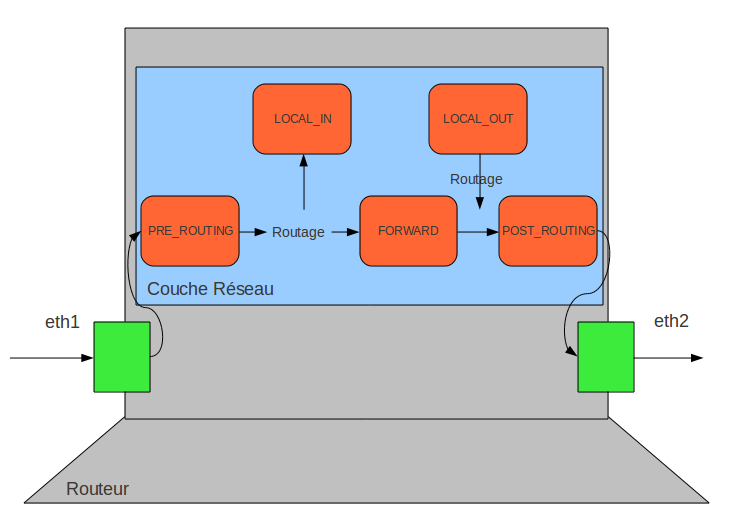
\includegraphics[scale=.5]{hooks.png}
	\caption{\label{hooks} Position des hooks Netfilter}
\end{figure}

Les paquets entrent dans le routeur par l'interface réseau eth1 et subissent des tests au niveau de la carte réseau. Ils traversent un premier 
hook, appelé \textit{NF\_IP\_PRE\_ROUTING}. Ensuite, après consultation de la table 
de routage, les paquets à destination du routeur sont dirigés vers un 
processus interne et passent par le deuxième hook, \textit{NF\_IP\_LOCAL\_IN}. 
Quant aux autres paquets, ils sont dirigés vers une interface de sortie 
et traversent successivement le troisième hook, \textit{NF\_IP\_FORWARD}, puis le 
quatrième, \textit{NF\_IP\_POST\_ROUTING}, avant de sortir du routeur par l'interface réseau eth2. Les paquets 
peuvent aussi être créés par le routeur lui-même. Ils passent alors 
par le hook \textit{NF\_IP\_LOCAL\_OUT}.

Netfilter va nous permettre, grâce aux hooks, d'ajouter des fonctionnalités au routeur 
sans toucher directement au code du noyau Linux. Afin d'utiliser Netfilter, il faut 
programmer un module en mode noyau. Les modules sont des morceaux de code écrits en 
langage C, pouvant être ajoutés ou retirés du noyau dynamiquement \cite{module1}. Ils apportent de 
nouvelles fonctionnalités au noyau. Dans notre cas, le module fournira des fonctions 
dites de callback qui seront automatiquement appelées lorsqu'un paquet traversera le 
hook associé à la fonction. Ces fonctions serviront à calculer les statistiques que 
nous devons fournir durant ce projet.
En ce qui concerne la programmation des modules en mode noyau sous Linux, elle est 
vraiment différente de celle en mode utilisateur. En effet, les bibliothèques sont 
plus restreintes et le débogage plus ardu, car le moindre accès mémoire invalide peut 
rendre le système inutilisable. Les détails techniques concernant ce type de programmation 
sont évoqués en annexe.

\section{Environnement de tests}

\subsection{Architecture}

Comme nous l'avons dit ci-dessus, la programmation en mode noyau peut avoir un grave 
impact sur le fonctionnement de l'ordinateur en cas de bug. De ce fait, nous avons 
décidé d'utiliser des machines virtuelles. Celles-ci vont également nous permettre 
de mettre aisément en place les interfaces réseaux nécessaires aux tests. La mise en 
place des machines virtuelles se fera grâce au logiciel VirtualBox\cite{virtbox}.

Dans un premier temps, on souhaite mettre en place une
architecture réseau simple, constituée de trois machines, la
figure \ref{topo} indiquant la topologie réseau suivie :
\begin{itemize}
	\item un émetteur;
	\item un routeur;
	\item et un récepteur.
\end{itemize}

\begin{figure}[!ht]
	\centering
	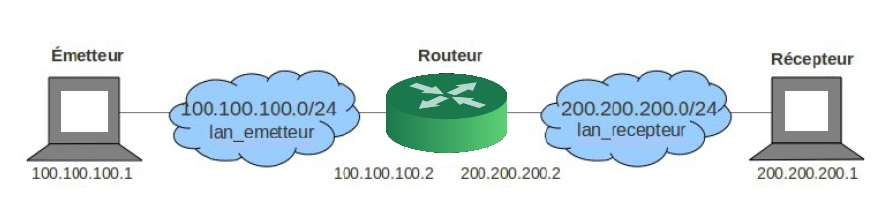
\includegraphics[scale=.5]{topo.jpg}
	\caption{\label{topo} Topologie du réseau}
\end{figure}

Pour cela nous utilisons trois machines virtuelles lancées sur la même machine hôte. 
Comme un routeur sert à faire transiter des données d'un réseau à un autre, deux
réseaux sont nécessaires ici : un sur lequel se trouve l'émetteur et un pour le récepteur.
VirtualBox permet de créer des réseaux locaux et les différentes machines virtuelles
 peuvent appartenir au réseau local que l’on souhaite \cite{virtualbx}. Nous créons donc deux réseaux locaux 
 comme dans le tableau \ref{reseaux1}.

\begin{figure}[!ht]
	\centering
	\begin{tabular}{c|c|c}
	Nom du réseau & Adresse réseau & Masque réseau\\
	lan\_emetteur & 100.100.100.0/24 & 255.255.255.0\\
	lan\_recepteur & 200.200.200.0/24 & 255.255.255.0\\
	\end{tabular}
	\caption{\label{reseaux1} Les deux réseaux}
\end{figure}

Sur chaque machine virtuelle, il faut configurer les interfaces réseaux et la table de routage. 
Ici l'émetteur peut atteindre le routeur. De même, le récepteur peut atteindre le routeur. 
En revanche, le routeur sert de passerelle entre l'émetteur et le récepteur.
Le routeur doit simplement être connecté aux deux réseaux.
Cela est possible car il dispose de plusieurs interfaces réseaux appelées eth0, eth1, eth2...
Chacune des deux interfaces du routeur doit donc être
connectée au bon réseau:
\begin{verbatim}
  # ifconfig eth1 100.100.100.2 netmask 255.255.255.0
  # ifconfig eth2 200.200.200.2 netmask 255.255.255.0
\end{verbatim}

Enfin, il ne faut pas oublier d'activer le transfert de
paquets :
\begin{verbatim}
  # echo 1 > /proc/sys/net/ipv4/ip_forward
\end{verbatim}

Du côté de l'émetteur, l'interface eth$0$ est reliée à
\textit{lan\_emetteur}, et il faut passer par 100.100.100.2
(c'est-à-dire l'interface eth$1$ du routeur) pour transmettre
des paquets à destination du réseau lan\_recepteur:
\begin{verbatim}
  # ifconfig eth0 100.100.100.1 netmask 255.255.255.0
  # route add -net 200.200.200.0 netmask 255.255.255.0 gw 100.100.100.2 eth0
\end{verbatim}

Côté récepteur, la configuration est analogue à celle de l'émetteur:
\begin{verbatim}
  # ifconfig eth0 200.200.200.1 netmask 255.255.255.0
  # route add -net 100.100.100.0 netmask 255.255.255.0 gw 200.200.200.2 eth0
\end{verbatim}

\subsection{Test de connectivité}
En guise de vérification, on essaie de \textit{pinger} le
récepteur depuis l'émetteur (figure \ref{ping1}):

\begin{figure}[!ht]
	\centering
	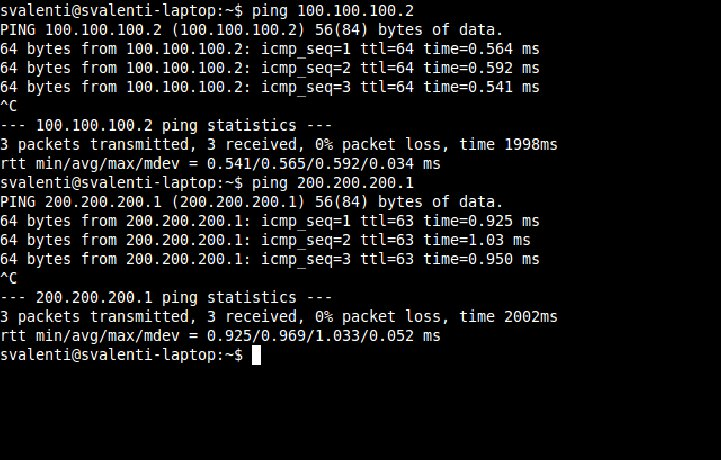
\includegraphics[scale=.5]{ping.jpg}
	\caption{\label{ping1} Émetteur et récepteur peuvent communiquer}
\end{figure}

La commande \textit{ping} n'est pas suffisante pour envoyer
des paquets dans le cadre de notre projet car elle utilise
le protocole ICMP et non le protocole TCP. Par conséquent,
nous avons cherché un outil utilisant le protocole TCP.
La commande \textit{iperf} permet d'envoyer entre un client et
un serveur des paquets TCP ou UDP. Nous l'avons donc utilisé
entre l'émetteur et le récepteur. Par défaut \textit{iperf}
utilise le protocole TCP.

Côté récepteur, on lance \textit{iperf} en mode serveur:
\begin{verbatim}
  # iperf -s
\end{verbatim}

et côté émetteur, on envoie des paquets sur le récepteur:
\begin{verbatim}
  # iperf -c 200.200.200.1
\end{verbatim}

L'option \textit{-i} d'\textit{iperf} peut être utilisée
pour fixer l'intervalle de temps entre les rapports
d'envois de paquets (mesure bande passante, $\ldots$).

\section{Calcul de la taille de la file d'attente avec Netfilter}
\`A présent, nous écrivons un module utilisant Netfilter. Les
fonctions de callback données par les hooks permettent
d'accéder à un \textit{struct sk\_buff} \cite{skbuff}. Cette structure représente
un paquet dans le noyau Linux. Il est ainsi possible de récupérer
les informations du datagramme telles que le protocole ou encore
l'adresse IP de destination.

Les fonctions de callback fournissent également deux structures
de type \textit{struct net\_device} : une pour l'interface réseau
d'entrée et une autre pour l'interface réseau de sortie. Avec
une telle structure, on peut connaître le nom de l'interface
grâce au champ \textit{net\_device.name}.

Cependant, ces structures ne sont pas toujours remplies par le noyau : cela 
dépend du hook dans lequel nous nous trouvons. En effet, dans le hook \textit{NF\_IP\_PRE\_ROUTING}, 
seule l'interface réseau d'entrée du paquet est connue. Dans le hook \textit{NF\_IP\_POST\_ROUTING}, 
c'est le contraire : seule l'interface de sortie est renseignée. En revanche, le hook \textit{NF\_IP\_FORWARD} 
connait les deux interfaces.
Pour déterminer où se trouve la file d'attente, nous devons travailler avec deux hooks : 
le premier hook doit se trouver en amont de l'emplacement supposé de la file d'attente et le second en aval. 
Dans le premier hook, la valeur de I de l'interface de sortie est incrémenté et, dans le second hook, 
la valeur de O de l'interface de sortie est incrémenté.
 
Après chaque opération, on met à jour la taille de la file
d'attente de l'interface de sortie en soustrayant l'Input Packets par l'Output Packets.

Les deux hooks pouvant accéder aux mêmes données en même temps,
il est indispensable de mettre en place un mécanisme de
synchronisation. Les hooks étant déclenchés par des interruptions,
il est impossible d'utiliser des mutex ou encore des sémaphores \cite{mutex}.
Le noyau fournit des spinlocks, jouant le même rôle, mais dans
un contexte d'interruptions. \cite{lock}

Les hooks concernant les paquets qui traversent le routeur sont :
\textit{NF\_IP\_PRE\_ROUTING}, \textit{NF\_IP\_FORWARD} et
\textit{NF\_IP\_POST\_ROUTING}. Parmi ces hooks, seuls
\textit{NF\_IP\_FORWARD} et \textit{NF\_IP\_POST\_ROUTING}
contiennent l'information sur l'interface de sortie dans la
structure \textit{net\_device}. Par conséquent, nous allons
tout d'abord chercher la taille de la file entre
\textit{NF\_IP\_FORWARD} et \textit{NF\_IP\_POST\_ROUTING}.

\subsection{\textit{NF\_IP\_FORWARD} et \textit{NF\_IP\_POST\_ROUTING}}
Pour commencer, les vitesses maximales des interfaces eth$1$ et
eth$2$ sont configurées de la même façon. Ainsi, on s'attend à
ce que la sortie des paquets soit fluide : nous ne nous attendons
pas à la création d'une file d'attente interne. L'exécution du module
utilisant ces deux hooks donne l'extrait de trace en
figure \ref{forwardpost}.

\begin{figure}[!ht]
	\centering
	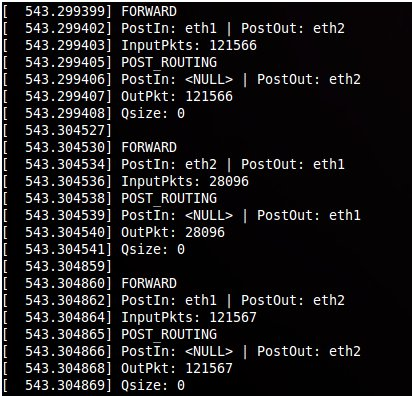
\includegraphics[scale=.5]{forward_post.jpg}
	\caption{\label{forwardpost} Trace obtenue entre FORWARD et POST}
\end{figure}

Après examination entière de la trace, on constate que Qsize
pour eth$1$ et Qsize pour eth$2$ sont constamment égaux à zéro.
On peut tout de même vérifier que le nombre de paquets entrants
est incrémenté correctement à chaque exécution de la fonction
de callback de \textit{NF\_IP\_FORWARD}. Quant au nombre de paquets
sortants, il est incrémenté correctement à chaque exécution de la
fonction de callback du hook \textit{NF\_IP\_POST\_ROUTING}.

À présent, on configure la bande passante maximale de l'interface
eth$2$ afin que la vitesse maximale soit de $10$ Mbits/seconde.
Pour cela, on utilise netem \cite{netem} avec la commande \textit{tc} (traffic control) \cite{tc1} \cite{tcman}.
Cette commande va agir sur le fonctionnement des files d’attente
en sortie d’une interface donnée.
\begin{verbatim}
  # tc qdisc add dev eth2 root handle 1: tbf rate 10mbit buffer 1600 limit 3000
  # tc qdisc add dev eth2 parent 1: handle 10: netem delay 3ms
\end{verbatim}
Pour limiter la bande passante, on utilise un Token Bucket Filter
(tbf) en précisant qu’on ne peut pas dépasser un débit de
$10$Mbits/seconde. Dans la pratique, la capacité des interface (C) est passée
en paramètre au chargement du module. Voici les rapports d'iperf en figure \ref{iperfe}

\begin{figure}[!ht]
	\centering
	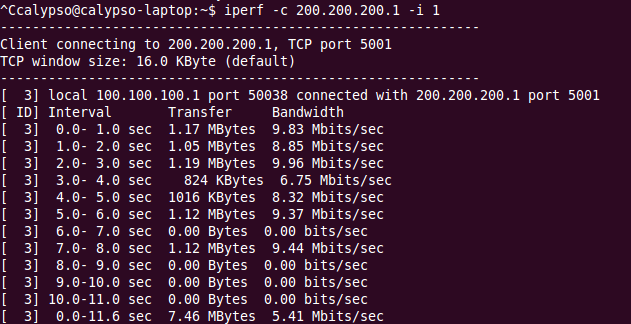
\includegraphics[scale=.5]{Capture-4.png}
	\caption{\label{iperfe} Rapport de bande passante d'iperf}
\end{figure}

Après avoir ainsi configuré la vitesse maximale,
nous nous attendons à obtenir une file d’attente non nulle.
Les résultats des tests effectués nous montrent que la taille
de la file d’attente est toujours nulle et qu'on n'a jamais
deux appels consécutifs au hook \textit{NF\_IP\_FORWARD}. 
Les paquets sont donc traités complètement : la file d'attente
ne se trouve pas entre les hooks
\textit{NF\_IP\_FORWARD} et \textit{NF\_IP\_POST\_ROUTING}.

Il nous faut donc regarder entre deux autres 
hooks : \textit{NF\_IP\_PRE\_ROUTING} et \textit{NF\_IP\_POST\_ROUTING}.

\subsection{\textit{NF\_IP\_PRE\_ROUTING} et \textit{NF\_IP\_POST\_ROUTING}}
L'interface de sortie n'étant pas disponible dans le hook \textit{NF\_IP\_PRE\_ROUTING},
il va nous falloir effectuer le routage à la main pour déterminer à quelle interface de sortie le paquet est destiné. Notre
objectif étant de chercher où se trouve la file, nous nous
contentons d'un routage manuel, avec des adresses IP fixes dans le code.

Nous obtenons finalement le même résultat que précédemment. 
Il semble donc qu'il soit impossible d'utiliser Netfilter pour
obtenir les statistiques. 

\subsection{Lecture des statistiques sur les cartes réseaux}
Grâce à une fonction du noyau, il est possible d’accéder à des
statistiques concernant les interfaces. La fonction \textit{dev\_get\_stats()}
définie dans \textit{linux/netdevice.h} fournit :
\begin{itemize}
	\item le nombre de paquets (ou octets) reçus sur une interface;
	\item le nombre de paquets (ou octets) transmis par une interface;
	\item le nombre d’erreurs;
	\item et le nombre de paquets \og dropped \fg.
\end{itemize}

Ces statistiques pourraient nous aider à calculer Qsize.
Effectivement, pour une interface de sortie donnée on connaît le
nombre de paquets transmis par cette interface.
Il faut se placer maintenant sur chacune des autres interfaces, et
comptabiliser le nombre de paquets entrants à destination
de notre interface de sortie. Cela est possible à condition
d'effectuer un routage des paquets pour connaître leur destination.

Cependant, les statistiques sur les cartes réseaux ne permettent pas de
différencier les paquets TCP des autres paquets, il faudrait
donc compter ceux-ci séparemment. De plus, le routage évoqué
est assez lourd. Il nous faut donc aller un peu plus loin dans le code.

\section{Analyse de la file d'attente au niveau de couche Liaison}

Après tous les tests que nous avons effectué précédemment, nous pouvons affirmer
 que la file d'attente contenant les paquets qui n'ont pas encore été traités ne
  se situe pas dans la couche Réseau du modèle 
  OSI. Par conséquent, nous allons tenter de l'analyser dans la couche
   inférieure du modèle OSI : la couche Liaison. Voici le schéma représentant
    les différentes phases du traitement d'un paquet :

Schéma !

\subsection{Les files d'attente avant routage}
Comme on peut le voir sur ce schéma issu de nos recherches, à la reception des paquets, ces derniers sont stockés dans une file d'attente appelée backlog \cite{10poin} ou ingress queue, dans la couche Liaison.
Lorsqu'un paquet entre, une interruption appelée \textit{NET\_RX\_SOFTIRQ} est levée. On peut choisir de traiter cette interruption grâce à un handler qui est une fonction appelée automatiquement lorsque l'interruption est levée. Nous avons donc essayé d'incrémenter le nombre de paquets dans ce handler et de continuer à le décrémenter  dans le hook \textit{NF\_IP\_POST\_ROUTING}. Malheureusement, le traitement des interruptions s'est avéré être plus compliqué que ce que nous pensions. Et nous n'avons pas voulu perdre de temps sur ce point puisque nos recherches nous ont appris que dans le cadre d'un routeur ERN, seul le taux d'occupation de la file d'attente entre en jeu. De telles files ne nous intéressent donc pas. 

\subsection{Les files d'attente après routage}

\subsubsection{File d'attente entre les fonctions dev\_queue\_xmit() et hard\_start\_xmit()}

Après le passage dans les hooks Netfilter, le paquet traverse la couche Liaison \cite{intel} \cite{stack}. \`A ce niveau, il y a une mise en file d’émission pour chaque interface de sortie. Cette file d’émission existe entre la fonction noyau \textit{dev\_queue\_xmit()} et la fonction \textit{hard\_start\_xmit()}. La première fonction enfile le paquet lorsqu’il passe de la couche Réseau à la couche Liaison. La deuxième fonction a pour but d’indiquer au noyau que les paquets ont été transmis à la carte réseau. Nous pouvons donc incrémenter le nombre de paquets au niveau de la fonction \textit{dev\_queue\_xmit()}, qui prend en compte l’interface de sortie.

Il n’est pas possible d’écrire un code modulaire pour ce type de manipulation.
Nous sommes contraints de modifier le code du noyau. Cela implique la compilation
d'un nouveau noyau, tâche assez lourde, et peu pratique : un module a le gros
avantage de ne pas être dépendant des sources du noyau.

\subsubsection{La compilation du noyau Linux}

Pour pouvoir compiler un noyau Linux \cite{compil}, il nous a fallu télécharger son code source. 
Tout d'abord, nous avons téléchargé sur le web une des versions les plus récentes. 
Mais, avec cette version, nous n'avions pas le bon fichier de configuration. De ce fait, 
la compilation du noyau prenait énormément d'espace sur le disque dur de la machine virtuelle 
et cela a rendu inutilisables un certain nombre de machines virtuelles malgré nos tentatives 
de leur allouer davantage d'espace disque. Cette étape nous a fait perdre beaucoup de temps.
Finalement, nous avons téléchargé un autre noyau moins récent grâce à la commande :
\begin{verbatim}
apt_get install linux-source-2.6.32
\end{verbatim}
Nous avons choisi la version 2.6.32 car c'est celle que nous avions sur nos machines, 
cela nous a permis de récupérer le fichier de configuration et la compilation prend beaucoup moins de place.
Après avoir téléchargé le noyau, il y a plusieurs étapes pour le compiler. 
Le téléchargement nous procure un fichier compressé, il faut donc le décompresser :
\begin{verbatim}
  # tar xvjf linux-2.6.32.tar.bz2
\end{verbatim}
Une fois la décompression effectuée, il faut placer le fichier de configuration trouvé dans /boot dans le dossier contenant le noyau et le renommer en .config.
\begin{verbatim}
  # cp /boot/config-2.6.32 .config
\end{verbatim}
Ensuite, il faut créer l'image binaire du noyau qui servira pour booter sur notre nouveau noyau :
\begin{verbatim}
  # make bzImage
\end{verbatim}
Les modules, qui comprennent notamment les pilotes utiles pour l'utilisation du clavier et de la souris par exemple, peuvent être compilés et installés :
\begin{verbatim}
  # make modules
  # make modules_install
\end{verbatim}
Enfin, on peut compiler et installer le noyau lui-même :
\begin{verbatim}
  # make
  # make install
\end{verbatim}
Pour pouvoir booter sur ce noyau ainsi installé, il faut taper la commande :
\begin{verbatim}
  # update-grub
\end{verbatim}
et redémarrer l'ordinateur.

\`A chaque modification d'un des fichiers sources du noyau, il faut refaire le make et le make install.

\subsubsection{Un premier essai dans la fonction dev\_queue\_xmit()}
En sortie, il existe une politique de gestion de files d'attente appelée qdisc.
Il s'agit d'une structure  comportant entre autre deux pointeurs sur fonction
enqueue et dequeue. Il existe une qdisc par interface de sortie.

Nous avons donc cherché à connaître le contenu effectif en paquets TCP de
la file d'attente. Il est clair que l'incrément du nombre de paquets TCP
doit se faire au début du corps de la fonction \textit{dev\_queue\_xmit()}
quand un appel à la fonction pointée par \textit{enqueue} est fait. Nous
avons aussi vu que la fonction \textit{dequeue} est appelée indirectement
par \textit{dev\_hard\_start\_xmit()} 
Cependant, le paquet peut très bien être dépilé de \textit{qdisc}, mais ne pas
être envoyé. Il est donc impératif de se placer à un niveau inférieur.

\subsubsection{Un second essai en utilisant la fonction dev\_hard\_start\_xmit()}

Comme on l'a dit précédemment, à chaque fois que la fonction \textit{dev\_queue\_xmit()}
est appelée, un paquet est mis en bufferisation. Nous avons vu que le décrément au
niveau du pointeur de fonction \textit{dequeue} ne fonctionnait pas : en fait,
le paquet est dépilé à la sortie de la couche transport, alors que la décrémentation
devrait plutôt être réalisée une fois le paquet mis sur le réseau. Par 
conséquent, nous avons cherché une fonction mettant le paquet dans la file
d'attente de la carte réseau. Il s'agit de la fonction \textit{ndo\_start\_xmit()}
appelée dans \textit{dev\_hard\_start\_xmit()}. 

En fait, chaque driver implémente une fonction permettant l'envoi de
paquets sur le réseau. Une solution naïve consisterait à chercher le
code du bon driver, et à y placer la décrémentation. Mais alors le
code ne fonctionnerait plus qu'avec un seul driver, à moins de tous
les modifier.

Les fonctions permettant de manipuler une carte Ethernet sont sous
Linux abstraites par une structure : ajouter un driver revient donc
à déclarer une structure et à remplir les différents champs avec
les fonctions adaptées à la carte.
La structure \textit{net\_device\_ops}, déclarée dans
\textit{linux/netdevice.h}, joue ce rôle:
\begin{verbatim}
struct net_device_ops {
    int (*ndo_init)(struct net_device *dev);
    void (*ndo_uninit)(struct net_device *dev);
    int (*ndo_open)(struct net_device *dev);
    int (*ndo_stop)(struct net_device *dev);
    netdev_tx_t (*ndo_start_xmit) (struct sk_buff *skb, struct net_device *dev);
    ...
};
\end{verbatim}

Et un driver, par exemple le driver e1000\footnote{Driver très répandu,
utilisé par la carte Intel. Il est présent notamment sur VirtualBox.},
l'utilise ainsi:
\begin{verbatim}
static const struct net_device_ops e1000_netdev_ops = {
    .ndo_open               = e1000_open,
    .ndo_stop               = e1000_close,
    .ndo_start_xmit         = e1000_xmit_frame,
    .ndo_get_stats          = e1000_get_stats,
    ...
};
\end{verbatim}

La fonction \textit{dev\_hard\_start\_xmit()}, située dans
\textit{net/core/dev.c}, est chargée de transmettre le paquet
à la carte. Après quelques tests à l'aide de \textit{printk} bien
placé, nous avons constaté que dans tous les cas, la fonction
est appelée, plus ou moins directement, et qu'elle contient 
un appel à \textit{ndo\_start\_xmit()} qui lancera la transmission réelle des paquets. La décrémentation de la
taille de la file peut donc être effectuée ici.

\section{Résultats}
En réglant la vitesse et la taille du buffer avec tc, on peut observer
une augmentation de Qsize : les paquets rentrent, mais ne sortent jamais.
L'hypothèse que nous avons par la suite vérifiée est que ces paquets
sont droppés par la carte : en regardant la valeur de retour (\textit{rc}) à

la  fin de \textit{dev\_queue\_xmit()}, on voit bien  qu'elle est à
\textit{NET\_XMIT\_DROP} au lieu de \textit{NET\_XMIT\_SUCCESS} à chaque
fois que Qsize n'est pas décrémenté
en sortie:
\begin{figure}[!ht]
	\centering
	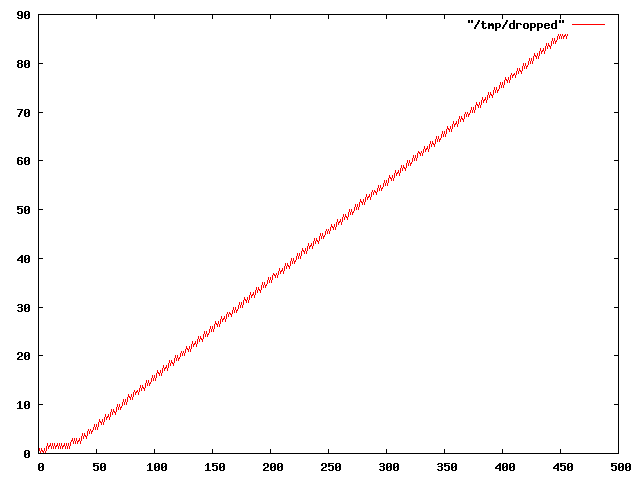
\includegraphics[scale=.5]{dropped.png}
	\caption{\label{dropped} Après réglage avec tc(1)}
\end{figure}

On pourrait très bien décrémenter Qsize à chaque paquet droppé : cela
permettrait de réinitialiser le compteur plutôt que de le laisser
grandir à chaque paquet non-envoyé, et cela resterait logique, dans le
sens où le paquet n'est plus dans la file d'attente.

Sans effectuer de  réglages, les paquets ne sont pas droppés, et, selon
la configuration de la carte, nous observons soit un
Qsize toujours à 0, soit un Qsize grandissant à l'occasion, mais se
réduisant par la suite:
\begin{figure}[!ht]
	\centering
	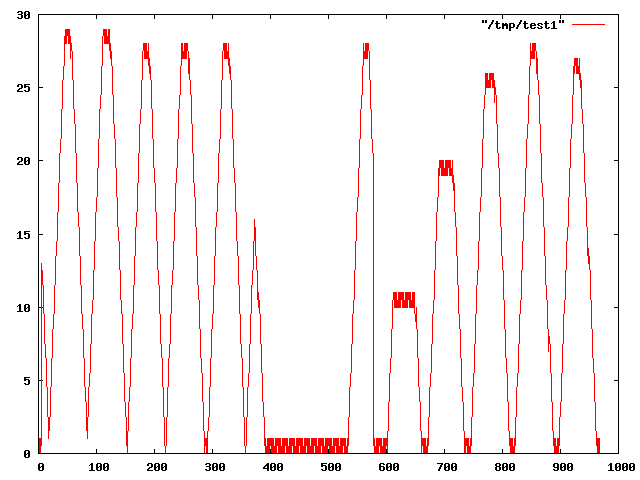
\includegraphics[scale=.5]{qsize_default.png}
	\caption{\label{qsize_default} Sans réglage}
\end{figure}

\section{Conclusion}
Durant ce projet, nous avons fourni une analyse de la taille de la file d'attente
réelle instantanée au sein d'un routeur ERN. Pour y parvenir, nous avons exploré 
différentes solutions avant d'aboutir à la solution finale utilisant la couche Liaison. 
Nos recherches nous ont fait appréhender un domaine jusqu'ici inconnu,
celui de la recherche. Elles nous ont également permis de développer nos connaissances
en réseau, en programmation en mode noyau et en virtualisation. 
Nos résultats sont exploitables par les chercheurs. Néanmoins, une statistique telle que
l'Input Traffic Rate devra être établie pour compléter le développement du framework
de notre routeur. Pour obtenir la vitesse, en sachant que l'on a déjà le nombre
de paquets entrants, il faudrait utiliser un timer.

\newpage
\appendix

\section{Compléments sur la programmation de modules Linux}
\subsection{Organisation générale}
Un module contient toujours deux fonctions respectivement exécutées
au chargement et au déchargement du module:
\begin{verbatim}
int
init_module(void)
{
    ...
}

void
cleanup_module(void)
{
    ...
}
\end{verbatim}

Les fonctions C \og classiques \fg\ ne sont plus disponibles, et
des équivalents en mode noyau viennent les remplacer : par exemple,
\textit{printf()} est remplacée par \textit{printk()}.

Pour charger/décharger un noyau, on peut utiliser au choix
\textit{insmod(8)} et \textit{rmmod(8)} ou encore \textit{modprobe(8)} pour charger et \textit{modprobe -r} pour décharger.

\subsection{Mise en place d'un hook Netfilter}
Un hook pour Netfilter est une fonction
\begin{verbatim}
unsigned int fun(unsigned int, struct sk_buff *, const struct net_device *,
	const struct net_device *, int (*)(struct sk_buff *));
\end{verbatim}

Elle est appelée dans un contexte d'interruptions, à chaque
fois qu'un paquet passe par le hook correspondant. Sont passés en arguments :
\begin{description}
	\item[struct sk\_buff *skb] le paquet;
	\item[const struct net\_device *in, *out] les interfaces d'entrées/sorties;
\end{description}

Typiquement, l'enregistrement du module se fait dans la fonction
\textit{init\_module()}:
\begin{verbatim}
static struct nf_hook_ops nfho;

...

int
init_module(void)
{
    nfho.hook     = fun;             /* handler function */
    nfho.hooknum  = NF_INET_FORWARD; /* emplacement du hook */
    nfho.pf       = PF_INET;
    nfho.priority = NF_IP_PRI_FIRST;   /* priorité */

    nf_register_hook(&nfho);
}
\end{verbatim}

et le déchargement dans \textit{cleanup\_module()}:
\begin{verbatim}
void cleanup_module()
{
    nf_unregister_hook(&nfho);
}
\end{verbatim}

\subsection{Synchronisation (spinlock)}
Les spinlocks sont un mécanisme de synchronisation utilisable
dans un contexte d'interruptions, comme c'est le cas pour les
hooks Netfilter. Nous nous sommes ici contentés de les utiliser
comme de simples verrous, ce que le code suivant résume:

\begin{verbatim}
#include <linux/spinlock.h>
static DEFINE_SPINLOCK(lock); 

{
    spin_lock_irq(&lock);    /* verouiller */
    /* code protégé */
    spin_unlock_irq(&lock);  /* dévérouiller */
}
\end{verbatim}

D'autres mécanismes comme les sémaphores ou les mutex sont
utilisables dans des cas moins particuliers.

\subsection{Module Netfilter}

\begin{verbatim}
/* Netfilter module for computing Qsize */

#ifndef __KERNEL__
        #define __KERNEL__
#endif
#ifndef MODULE
        #define MODULE
#endif

#include <linux/version.h>
#include <linux/module.h>
#include <linux/moduleparam.h>
#include <linux/kernel.h>
#include <linux/netfilter.h>
#include <linux/netfilter_ipv4.h>
#include <linux/init.h>
#include <linux/skbuff.h>
#include <linux/tcp.h>
#include <asm/io.h>
#include <linux/inet.h>
#include <linux/vmalloc.h>
#include <net/ip.h>

#include <net/route.h>

#include <linux/spinlock.h>

#if LINUX_VERSION_CODE >= KERNEL_VERSION(2,6,16)
#include <linux/in.h>
#include <linux/ip.h>
#endif

#define NB_INTFS 3
#define NB_STATS 4

/* Args */
static int outputRate_eth1 = 1000; 
static int outputRate_eth2 = 10; 
module_param(outputRate_eth1, int, 0);
module_param(outputRate_eth2, int, 0);

static DEFINE_SPINLOCK(lock); 

static int stats_packets[NB_INTFS][NB_STATS] = { { 0 } };

/* This is the structure we shall use to register our function */
static struct nf_hook_ops nfho_forward;
static struct nf_hook_ops nfho_post;
static struct nf_hook_ops nfho_pre;

/* Name of the interface we want to drop packets from */
struct sk_buff *sock_buff;
struct iphdr *ip_header;
struct tcphdr *tcp_header;

inline int hash_index(const char* name_intf) { 
	return name_intf[strlen(name_intf) - 1] - '0'; 
}

/* Hook function: FORWARD */
unsigned int hook_func_forward(unsigned int hooknum, struct sk_buff *skb, const struct net_device *in, const struct net_device *out, int (*okfn)(struct sk_buff *)) {

	int index;
	sock_buff = skb; // Ok, useless but ...
	
	if (!sock_buff) { 
		return NF_ACCEPT; 
	}
	ip_header = (struct iphdr *) skb_network_header (sock_buff);
	if (!ip_header) { 
		return NF_ACCEPT; 
	}
	if (ip_header->protocol != 6) { 
		return NF_ACCEPT; 
	}
	tcp_header = (struct tcphdr *) skb_transport_header (sock_buff);
	if (!tcp_header) { return NF_ACCEPT; }
	
	return NF_ACCEPT;
}

/* Hook function: POST */
unsigned int hook_func_post(unsigned int hooknum, struct sk_buff *skb, const struct net_device *in, const struct net_device *out, int (*okfn)(struct sk_buff *)) {

	int index;
	sock_buff = skb; // Ok, useless but ...
	
	if (!sock_buff) { 
		return NF_ACCEPT; }
	ip_header = (struct iphdr *) skb_network_header (sock_buff);
	if (!ip_header) { 
		return NF_ACCEPT; 
	}
	if (ip_header->protocol != 6) { 
		return NF_ACCEPT; 
	}
	tcp_header = (struct tcphdr *) skb_transport_header (sock_buff);
	if (!tcp_header) { 
		return NF_ACCEPT; 
	}
	
	printk(KERN_CRIT "POST");
	printk(KERN_CRIT "PostIn: %s | PostOut: %s", in->name, out->name);

	index = hash_index(out->name);

	spin_lock_irq(&lock);
	stats_packets[index][1]++; // O++
	stats_packets[index][2] = stats_packets[index][0] - stats_packets[index][1]; // qsize = I - O
	printk(KERN_CRIT "OutPkt: %d\n", stats_packets[index][1]);
	printk(KERN_CRIT "Qsize: %d\n", stats_packets[index][2]);
	spin_unlock_irq(&lock);

	return NF_ACCEPT;
}

/* Hook function: PRE */
unsigned int hook_func_pre(unsigned int hooknum, struct sk_buff *skb, const struct net_device *in, const struct net_device *out, int (*okfn)(struct sk_buff *)) {

	int rc = 51;
	int index = 42;
	__be32 src, dst;
	u8 tos;

	// Ok, useless but ...
	sock_buff = skb;
	
	if (!sock_buff) { 
		return NF_ACCEPT; 
	}
	ip_header = (struct iphdr *) skb_network_header (sock_buff);
	if (!(ip_header)) { 
		return NF_ACCEPT; 
	}
	if (ip_header->protocol != 6) { 
		return NF_ACCEPT; 
	}
	tcp_header = (struct tcphdr *) skb_transport_header (sock_buff);
	if (!tcp_header) { 
		return NF_ACCEPT; 
	}
	
	printk(KERN_CRIT "\nPRE");
	printk(KERN_CRIT "PreIn: %s | PreOut: %s", in->name, out->name);

	// Tests routage propre
	src = ip_header->saddr;
	dst = ip_header->daddr;
	tos = ip_header->tos;
	rc = ip_route_input(skb, dst, src, tos, in);
	printk(KERN_CRIT "Route: %d", rc);

	if (ip_header->daddr == 29935816) { // Target: 200.200.200.1 via eth2
		index = hash_index("eth2");
	} else if (ip_header->daddr == 23356516) { // Target: 100.100.100.1 via eth1
		index = hash_index("eth1");
	}
	if (index == 42) {
		return NF_ACCEPT;
	}
	
	spin_lock_irq(&lock);
	stats_packets[index][0]++;
	//stats_packets[index][2] = stats_packets[index][0] - stats_packets[index][1]; // qsize = I - O
	printk(KERN_CRIT "InputPkts: %d\n", stats_packets[index][0]);
	//printk(KERN_CRIT "Qsize: %d\n", stats_packets[index][2]);
	spin_unlock_irq(&lock);

	return NF_ACCEPT;
}

/* Initialisation routine */
int init_module()
{

	/* Fill in our hook structure */
	nfho_forward.hook     = hook_func_forward;         /* Handler function */
	nfho_forward.hooknum  = NF_INET_FORWARD; /* NF_IP_FORWARD */
	nfho_forward.pf       = PF_INET;
	nfho_forward.priority = NF_IP_PRI_FIRST;   /* Make our function first */

	/* Fill in our hook structure */
	nfho_post.hook     = hook_func_post;         /* Handler function */
	nfho_post.hooknum  = NF_INET_POST_ROUTING; /* NF_IP_FORWARD */
	nfho_post.pf       = PF_INET;
	nfho_post.priority = NF_IP_PRI_FIRST;   /* Make our function first */

	/* Fill in our hook structure */
	nfho_pre.hook     = hook_func_pre;         /* Handler function */
	nfho_pre.hooknum  = NF_INET_PRE_ROUTING; /* NF_IP_FORWARD */
	nfho_pre.pf       = PF_INET;
	nfho_pre.priority = NF_IP_PRI_FIRST;   /* Make our function first */

	printk(KERN_CRIT "Go ahead\n");
	nf_register_hook(&nfho_forward);
	nf_register_hook(&nfho_post);
	nf_register_hook(&nfho_pre);

	//stats_packets[1][1] = outputRate_eth1;
	//stats_packets[2][1] = outputRate_eth2;

	return 0;
}
/* Cleanup routine */
void cleanup_module()
{
	nf_unregister_hook(&nfho_forward);
	nf_unregister_hook(&nfho_post);
	nf_unregister_hook(&nfho_pre);
}

MODULE_LICENSE("GPL");

\end{verbatim}

\subsection{Fonctions modifiées du noyau}

\newpage
\bibliographystyle{ieeetr}
\bibliography{docs}

\textbf{Autre documentation consultée:}
\begin{itemize}
	\item Commande mii-tool (configuration vitesse) : 
	http://www.cyberciti.biz/faq/linux-change-the-speed-and-duplex-settings-of-an-ethernet-card/
	\item Source du noyau : http://lxr.linux.no/
\end{itemize}

\end{document}
